\chapter{The human microbiome and nonalcoholic fatty liver disease}

\section{Introduction}
Non alcoholic fatty liver disease (NAFLD) has been on the rise along with obesity, affecting a fifth to a third of the North American population \cite{preiss2008non}. Most people with NAFLD remain asymptomatic, however, in up to a third of patients NAFLD can progress to nonalcoholic steatohepatitis (NASH), causing inflammation and scarring (fibrosis) in the liver, and decreasing the 5 year survival rate to 67\% \cite{propst1995prognosis}. It is thus important to shed some light on the process by which people progress from NAFLD to NASH to find interventions that prevent NASH.

\subsection{NASH progression risk}
There are several known genetic and chemical factors that increase the risk of progression to NASH in animal models and humans.

\paragraph{Mouse}\mbox{}\\
In mice non alcoholic fatty liver disease is often modelled with a methionine/choline-deficient diet (MCD), which induces steatohepatitis in wildtype mice. Mice with a toll-like receptor 4 knockout had lower lipid and injury accumulation markers when fed a MCD diet \cite{rivera2007toll}.

\paragraph{Rat}\mbox{}\\
In rats liver fibrosis can be induced by drugs. One study found that male rats were more prone to this induced liver fibrosis than female rats. Fibrosis biomarkers were reduced when the male rats were dosed with estradiol, and increased when the male rats were additionally given an estradiol-neutralizing antibody. Female rats who had their ovaries removed similarly lost the protective effect \cite{yasuda1999suppressive}. From this, hormones are also a factor in nonalcoholic fatty liver disease progression.

\paragraph{Human}\mbox{}\\
In humans, the I148M variant of the Patatin-Like Phospholipase Domain Containing 3 gene (PNPLA3) correlates with a 3.2 fold increased risk of progression to NASH from NAFLD when homozygous, compared to to patients without the variant \cite{sookoian2011meta}. The heterozygous gene was found to be associated with fatty liver disease in genome wide association studies, but some additional studies have faileid to replicate the relationship with NASH \cite{sookoian2011meta}.

On the epigenetic level, many genes are differentially methylated in advanced NAFLD compared to mild NAFLD. 11\% of genes are differentially hypomethylated in advanced NAFLD (compared to 3\% hypermethylated), leading to increased expression \cite{murphy2013relationship}. In advanced NASH specifically, some tissue repair genes were hypomethylted while some metabolism pathways such as 1-carbon metabolism were hypermethylated. However, only 7\% of the differentially methylated genes were found to be differentially transcribed \cite{murphy2013relationship}.

On a metabolite level, Raman et al. found differences in the number of volatile organic compounds detected in patients with NAFLD compared to obese patients without NAFLD \cite{raman2013fecal}. Reactive oxygen species have also been implicated in NASH due to their involvement in the mechanism of steatohepatitis-inducing drugs \cite{berson1998steatohepatitis}.

 The microbiome is thought to have an effect on host digestion and absorption of nutrients \cite{gill2006metagenomic}. Fermenters produce short chain fatty acids, which make up 10\% of the calories in a Western diet \cite{mcneil1984contribution} Some groups claim a link between ethanol-producing gut bacteria and NAFLD \cite{zhu2013characterization} \cite{jiang2015dysbiosis}, however the evidence was inconclusive since no multiple test correction was performed.

\subsection{Data}
Applying next generation sequencing techniques to microbiome research is a relatively new field that has yet to set data analysis standards. There are some considerations that should be made when constructing a data analysis strategy.

\paragraph{Data is multivariate}\mbox{}\\
Generally experiments of this nature typically have low sample sizes due to budget constraints, sample collection difficulties, patient compliance, and other issues.

As a result, the number of taxa or gene functions comparisons made are often a magnitude larger than the sample size. This is known in statistics as having more variables than observations, or having fat data. The higher the ratio of variables to observations are, the less likely standard statistical techniques are to be reliable \cite{osborne2004sample}.

Researchers should include multiple test corrections to ensure that the results they are reporting are true, at the expense of having p-values less than 0.05. Unfortunately many studies have been published in high impact journals without multiple test corrections, including a famous paper linking the gut microbiome to autism published in Cell \cite{hsiao2013microbiota}.

\paragraph{Data is compositional}\mbox{}\\
In both gene tag sequencing and metagenomic sequencing experiments, the data is in the form of a list of counts per feature, with the features composing an aspect of the microbiome for each sample. This is compositional data. The total number of reads yielded by the sequencing platform is often platform-dependant and not biologically relevant.

This constrained sum causes the abundance of different taxa to appear to be negatively correlated with each other when analyzed by conventional statistics. When one taxa increases in abundance, the counts detected in other taxa decrease in abundance, even if the taxa are not decreasing in abundance biologically.

Compositional data should be analyzed in a compositional way. In Euclidean space, data points can increase or decrease freely. Compositional data is under a sum constraint, and exist in a non-Euclidean space known as the Aitchison simplex \cite{aitchison1982statistical}. Data transformations such as the centered log ratio can be performed to put the data into Euclidean space, so that it can be analyzed with standard statistical methods that depend on Cartesian coordinates and linear relationships.

However, these techniques are not yet mainstream in the field, resulting in a high number of conclusions made that are not reproducible.

\subsection{Literature}
Several papers have already been published in the literature on the topic of NAFLD and the gut microbiome:

\begin{figure}[h]
\begin{center}
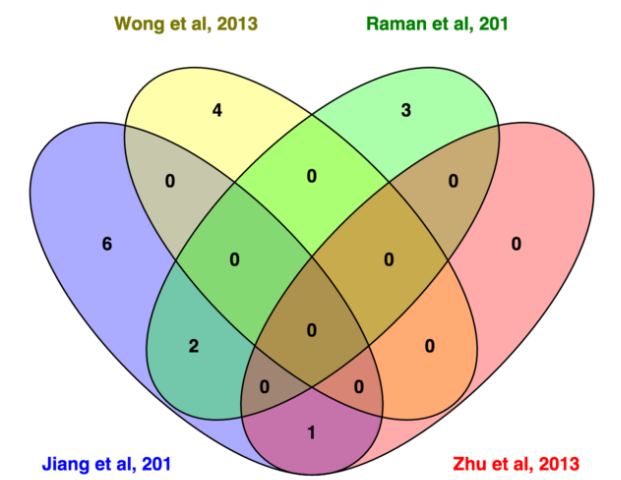
\includegraphics[width=0.7\textwidth]{nafld_papers.png}
\caption[Venn diagram of genera found to be differentially abundant by different studies between NASH/NAFLD and healthy controls.]{\textbf{Venn diagram of genera found to be differentially abundant by different studies between NASH/NAFLD and healthy controls.} Only 3 out of the 16 genera claimed to be differentially abundant were found in two studies: members of the \textit{Escherichia} genus were found in the Zhu \cite{zhu2013characterization} and Jiang \cite{jiang2015dysbiosis} studies, and members of the \textit{Lactobacillus} and \textit{Oscillibacter} genus were found in the Jiang \cite{jiang2015dysbiosis} and Raman \cite{raman2013fecal} studies.}
\end{center}
\label{nafld_fig1}
\end{figure}

\paragraph{Jiang et al, 2015 \cite{jiang2015dysbiosis}}\mbox{}\\
\textbf{Study:} This group compared 53 NAFLD patients with 32 healthy controls. The NAFLD patients had a significantly higher BMI ($P<0.01$).\\
\textbf{Sequencing:} Each sample had an average of 0.6 million reads, from sequencing the V3 region of the 16S rRNA gene on the Illumina sequencing platform.\\
\textbf{Analysis:} The reads were annotated with the Ribosomal Database Project \cite{cole2009ribosomal} and differential abundance was determined using Projection on Latent Structures - Discriminant Analysis (PLS-DA) methods.\\
\textbf{Results:} They found a relative increase in members of the \textit{Lentisphaerae} phyla and the \textit{Oscillibacter} and \textit{Flavonifractor} genera in the healthy group, and a relative increase in members of the \textit{Clostridium XI}, \textit{Anaerobacter}-related, \textit{Streptococcus}, and \textit{Lactobacillus} genera in the NAFLD group.

\paragraph{Zhu et al, 2013 \cite{zhu2013characterization}}\mbox{}\\
\textbf{Study:} This group compared 16 non-obese controls, 25 obese patients, and 22 NASH patients. All of the patients were pediatric, and the NAFLD group all had a BMI higher than the 85th percentile while the healthy group had BMIs less than the 85th percentile.\\
\textbf{Sequencing:} A 16S rRNA gene tag sequencing experiment was performed and reads were sequenced in a 454 pyrosequencer.\\
\textbf{Analysis:} This group used MG-RAST \cite{meyer2008metagenomics} and QIIME \cite{caporaso2010qiime}.\\
\textbf{Results:} Note that in the PCoA plot, there is only 11\% variance explained by the first component, and they had to plot the first component with the 3rd component (3\% variance explained) to show the group separation. By comparing the average absolute read count for each taxa in each group, this group found that members of the \textit{Proteobacteria} phylum, the \textit{Enterobacteriaceae} family, and the \textit{Escherichia} genus had significantly higher average counts in NASH patients compared to obese patients and healthy controls.

\paragraph{Raman et al, 2013 \cite{raman2013fecal}}\mbox{}\\
\textbf{Study:} This group compared 30 NAFLD patients with 30 healthy controls. All the healthy controls had a BMI less than 25 while all the NAFLD patients had a BMI greater than 30.\\
\textbf{Sequencing:} The 16S rRNA gene was amplified and sequenced with 454 pyrosequencing, yielding 2000 reads per sample.\\
\textbf{Analysis:} Reads were annotated with the Ribosomal Database Project \cite{cole2009ribosomal}. UniFrac analysis was performed with QIIME \cite{caporaso2010qiime}, and differential abundance was tested with Metastats \cite{paulson2011metastats}.\\
\textbf{Results:} They found a relative increase in members of the \textit{Lactobacillus}, \textit{Robinsoniella}, \textit{Roseburia}, and \textit{Dorea} genus in NASH patients and a relative increase in members of the \textit{Oscillibacter} in healthy patients.

\paragraph{Wong et al, 2013 \cite{wong2013molecular}}\mbox{}\\
\textbf{Study:} This group compared 16 NASH patients with 22 healthy controls.\\
\textbf{Sequencing:} They amplified the V1-V2 variable region of the 16S rRNA gene with pyrosequencing, yielding 4-11 thousand reads per sample.\\
\textbf{Analysis:} Reads were clustered with UCLUST \cite{edgar2010search} and annotated with the Ribosomal Database Project \cite{cole2009ribosomal}.\\
\textbf{Results:} Members of the the genera \textit{Parabacteroides} and \textit{Allisonella} were found to be relatively increased in NASH patients, while members of the genera \textit{Faecalibacterium} and \textit{Anaerosporobacter} were relatively increased in healthy controls.

\paragraph{Boursier et al, 2015 \cite{boursier2016severity}}\mbox{}\\
\textbf{Study:} This group compared 30 patients with F0 or F1 fibrosis to 27 patients with F2 or greater fibrosis, 35 of which had NASH\\
\textbf{Sequencing:} A gene tag experiment was performed on the V4 region of the 16S rRNA gene, and sequenced on an Illumina platform, yeilding an average of 0.2 million reads per sample.\\
\textbf{Analysis:} Reads were annotated with the Greengenes database \cite{desantis2006greengenes}, and differential abundance was measured by Mann-Whitney's test. A metagenomic imputation was performed with PiCrust \cite{langille2013predictive}, annotated with KEGG \cite{kanehisa2000kegg}, and analysed with LEfSE \cite{segata2011metagenomic}.\\
\textbf{Results:} A relative increase in members of the \textit{Bacteroides} phylum and a relative decrease in members of the \textit{Prevotella} phylum was found in NASH, compared to healthy controls. From the metagenomic imputation, the gut microbiome of NASH patients was found to be significantly enriched functional categories related to carbohydrate, lipid, amino acid, and secondary metabolism.

Many of the studies had healthy controls with a lower BMI, so it is difficult to separate whether the differences found are related to NAFLD progression or obesity.

Fig.~\ref{nafld_fig1} shows a Venn diagram illustrating the inconsistency of the literature on the gut microbiome and NAFLD. Of these, only Raman et al \cite{raman2013fecal} reported using a multiple test correction.

Since these five studies do not form a consistent story about the gut microbiome and NAFLD, we conducted own analysis rigorously, such that our results are replicable. Additionally, we generate the first deeply sequenced metagenomic sample set to examine functional capabilities in this disease.

\FloatBarrier

\section{Methods}
In total, 67 samples were collected: 29 from patients with nonalcoholic steatohepatitis (NASH), 14 from patients with simple steatosis (SS), and 24 from healthy controls. The median BMIs were 26.70, 27.34, and 32.06, and the median ages were 36, 49, and 46.5 for healthy, SS, and NASH respectively.

DNA extraction was performed with the \href{http://omegabiotek.com/store/product/stool-dna-kit/}{E.Z.N.A.® Stool DNA Kit}, and the protocol was followed with the addition of lysozyme with an extra 30 minute incubation at 37 degrees Celcius, between steps 2 and 3.

\subsection{16S rRNA gene tag experiment}

DNA was amplified by PCR using the Earth Microbiome V4 primer set \cite{caporaso2012ultra}, with the addition of combinatorial in-line barcodes so that all the samples could be sequenced in the same sequencing run \cite{gloor2010microbiome}. The DNA was sequenced on the Illumina MiSeq platform with paired end 220 nucleotide reads, producing 25 million reads in total.

Reads were overlapped with Pandaseq \cite{masella2012pandaseq}, clustered into Operational Taxonomic Units (OTUs) using UCLUST \cite{edgar2010search}, and annotated with the SILVA database \cite{quast2013silva} using mothur \cite{schloss2009introducing}, producing a table of counts per operational taxonomic unit per sample. Twelve milion (48\%) of the reads were succesfully overlapped and annotated into 232 OTUs. Differential abundance was analyzed using ALDEx2 \cite{fernandes2014unifying}.

A generalized workflow for processing 16S rRNA gene sequencing reads is available at \url{https://github.com/ggloor/miseq_bin}. The workflow for the 16S rRNA gene tag experiment analysis from the count table stage is on GitHub: \url{https://github.com/ruthgrace/nafld_metaphlan_pca}.

\subsection{MetaPhlAn}

MetaPhlAn (Metagenomic Phylogenetic Analysis) \cite{segata2012metagenomic} is a piece of software that allows one to infer the taxa present based on the metagenomic sequencing experiment. We used this to generate a count table per taxa per sample, and will compare it to our experimental results from the 16S rRNA gene tag sequencing experiment.

The MetaPhlAn tutorial (\url{https://bitbucket.org/nsegata/metaphlan/wiki/MetaPhlAn_Pipelines_Tutorial}) was followed, using an additoinal marker_counts option in the merge_metaphlan_tables.py step to produce a count table instead of a relative abundance table. The workflow for the MetaPhlAn analysis from the count table stage is on GitHub: \url{https://github.com/ruthgrace/nafld_metaphlan_pca}.

\subsection{Metagenomic experiment}

\textsc{\begin{table}[!ht]
% \begin{adjustwidth}{-2.25in}{0in} % Comment out/remove adjustwidth environment if table fits in text column.
\begin{tabular}{|l|}
\hline
\bf{Study inclusion criteria}\\ \hline
BMI $>$ 40 kg/m2\\
or BMI $>$ 35-40 kg/m2 with severe weight loss responsive comorbidities,\\
i.e. DM2, hypertension, hyperlipidemia, sleep apnea\\
and/or gastroesophageal reflux disease\\
or physical problems interfering with lifestyle\\
and who have been assessed by the multidisciplinary bariatric team\\
as suitable candidates for laparoscopic RYGB\\ \hline
Male and female\\ \hline
Age 18 years or older\\ \hline
Alcohol consumption <20g/d\\ \hline
If known to have hyperlipidemia or DM2,\\
need to be stable drug regimen for at least 3 months prior to study entry\\ \hline
\bf{Study exclusion criteria}\\ \hline
Liver disease of other etiology\\ \hline
Advanced liver disease\\
(need for liver transplantation in one year\\
or complications such as variceal bleeding, ascites or jaundice)\\ \hline
Abnormal coagulation or other reasons contraindicating a liver biopsy\\ \hline
Medications known to precipitate steatohepatitis 6 months prior to entry\\ \hline
Regular intake of non-steroidal anti-inflammatory drugs;\\
prebiotics, probiotics or antibiotics, ursodeoxycholic acid\\
or any experimental drug in the 3 months prior to study entry\\ \hline
Type 1 diabetes\\ \hline
Chronic gastrointestinal diseases\\ \hline
Previous gastrointestinal surgery modifying the anatomy (prior to bariatric surgery)\\ \hline
Smoking\\ \hline
Pregnancy or breastfeeding\\ \hline
Patients not tolerating Optifast,\\
which is a standard weight loss diet given to all patients pre-bariatric surgery\\ \hline
\end{tabular}
\caption[List of overall study inclusion and exclusion criteria.]{ \textbf{List of overall study inclusion and exclusion criteria.} This table lists the inclusion and exclusion criteria for the 16S rRNA gene tag experiment.}
\label{nafld_table_1}
% \end{adjustwidth}
\end{table}}

\textsc{\begin{table}[!ht]
% \begin{adjustwidth}{-2.25in}{0in} % Comment out/remove adjustwidth environment if table fits in text column.
\begin{tabular}{|l|}
\hline
\bf{Study inclusion criteria}\\ \hline
NASH severity\\ \hline
\bf{Study exclusion criteria}\\ \hline
Took antibiotics at any point\\ \hline
Started Optifast diet early\\ \hline
Sample not frozen immediately after collection\\ \hline
Blood glucose over 7.8 mmol/l\\ \hline
\end{tabular}
\caption[List of inclusion and exclusion criteria for metagenomic study.]{ \textbf{List of inclusion and exclusion criteria for metagenomic study.} Patients were selected for the metagenomic study out of the patients selected for the 16S rRNA gene tag sequencing study with the following criteria. Ten healthy and ten patients with NASH were selected in total.}
\label{nafld_table_1}
% \end{adjustwidth}
\end{table}}

A metagenomic sequencing experiment was performed using total bacterial DNA from 10 healthy controls and 10 of the patients with NASH. Samples from healthy patients were selected to exclude confounding factors. Samples from NASH patients were selected for the most extreme NASH phenotype, and had higher effect sizes in the 16S rRNA gene tag experiment than the full NASH group.

The DNA was sequenced on the Illumina HiSeq platform, with single end 100 nucleotide reads. Samples were barcoded and sequenced on the same sequencing run. After sequencing, the reads were quality filtered and demultiplexed to separate the reads for each sample, yielding nearly 2 billion reads in total.

We used a two pronged strategy to annotate the reads:

First, we created a reference library using the inferred taxa from the 16S rRNA gene tag experiment. For each genus observed we randomly picked 10 strain genomes from the NCBI bacterial genome database. For genera with less than 10 fully sequenced representatives, we selected all available genomes. The library was made with 1134 genomes from 104 bacterial genera. The open reading frame (ORF) library was then clustered at 99\% identity for each genus using CD-HIT \cite{li2006cd} to decrease the number of ORFs in the library from 3,495,887 to 2,256,844. Annotation was performed with the SEED database \cite{overbeek2005subsystems}, and sequenced reads were mapped onto this ORF library. Out of approximately 2 billion reads total, 58.5 million (30.6\%) were mapped by this method, over 5836 unique SEED hierarchy annotations. The primary limitation of this method is a lack of annotated bacterial sequences. The code for the \href{https://github.com/ruthgrace/make_functional_mapping_library}{reference library creation} and \href{https://github.com/ruthgrace/mapping_library_annotated_counts}{annotation} is on GitHub.

Second, we assembled the reads per sample de novo using Trinity \cite{haas2013novo}, producing 8847816 sequences, and removed sequences that matched our reference library with 90\% identity as determined by BLAST \cite{altschul1990basic}, leaving 5,876,423 sequences. [FILL IN THIS] of these assembled sequences were successfully annotated with the SEED database \cite{overbeek2005subsystems}, and sequenced reads were mapped onto this. [FILL IN THIS] additional reads were annotated by this method, over [FILL IN THIS] unique SEED hierarchy annotations. The code for the custom assembly pipeline is on \href{https://github.com/ruthgrace/exploring_nafld_assembly}{GitHub}. The data from both prongs was amalgamated into a single table of counts per annotation per sample.

Differential abudance was analyzed using ALDEx2 \cite{fernandes2014unifying}. A full description of the workflow for this process is included in Appendix ~\ref{AppA}.

\FloatBarrier

\section{Results}

\subsection{16S rRNA gene tag experiment}
The top four genus detected by 16S rRNA gene sequencing (excluding unclassified bacteria) were: \textit{Bacteroides}, \textit{Faecalibacterium}, \textit{Blautia}, and \textit{Pseudobutyrivibrio} (Fig.~\ref{nafld_16s_barplot}).

\begin{figure}[h]
\begin{center}
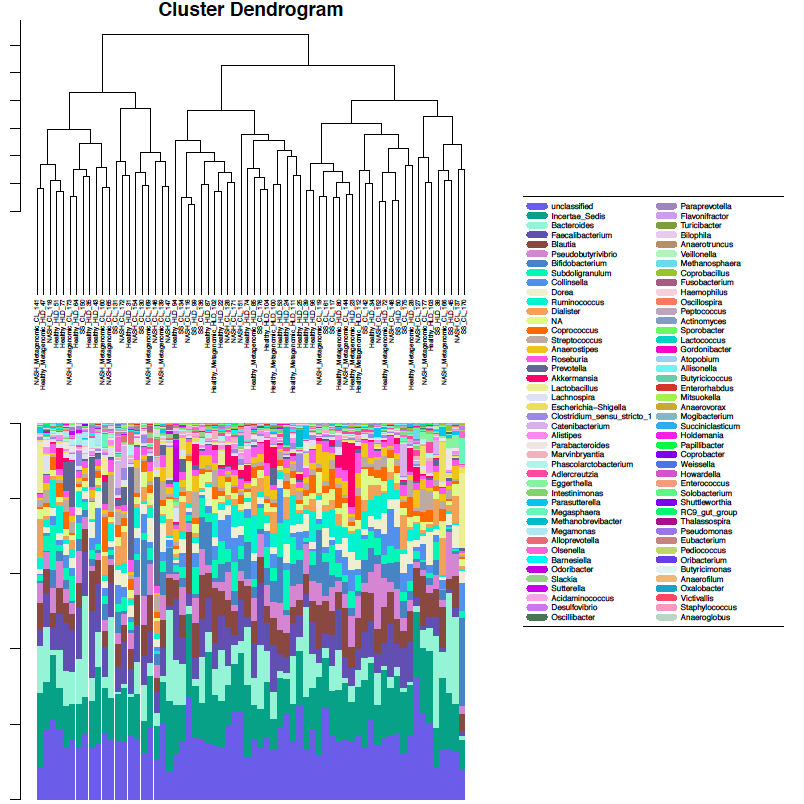
\includegraphics[width=0.95\textwidth]{16s_genus_barplot.png}
\caption[Bar plot of 16S rRNA gene tag sequencing experiment.]{\textbf{Bar plot of 16S rRNA gene tag sequencing experiment.} Each column of this bar plot represents one sample, and each color represents one bacterial genus. Genus are listed in the legend in order of decreasing total abundance across all samples. Samples do not cluster according to their condition (healthy, simple steatosis, or nonalcoholic steatohepatitis). Note that OTUs that mapped to unclassified or \textit{Incertae Sedis} were removed, and these made up just over a third of the total abundance.}
\end{center}
\label{nafld_16s_barplot}
\end{figure}

No obvious structure or separation is evident from the principal components analysis in Fig.~\ref{nafld_fig2} or the principal coordinate analysis in Fig.~\ref{nafld_16s_biplot}. Furthermore the variance explained by each principal component axis is not notably high, indicating a rather uniform data set. Additionally, no OTUs are significantly differentially abundant between groups (Fig.~\ref{nafld_fig3})

\begin{figure}[h]
\begin{center}
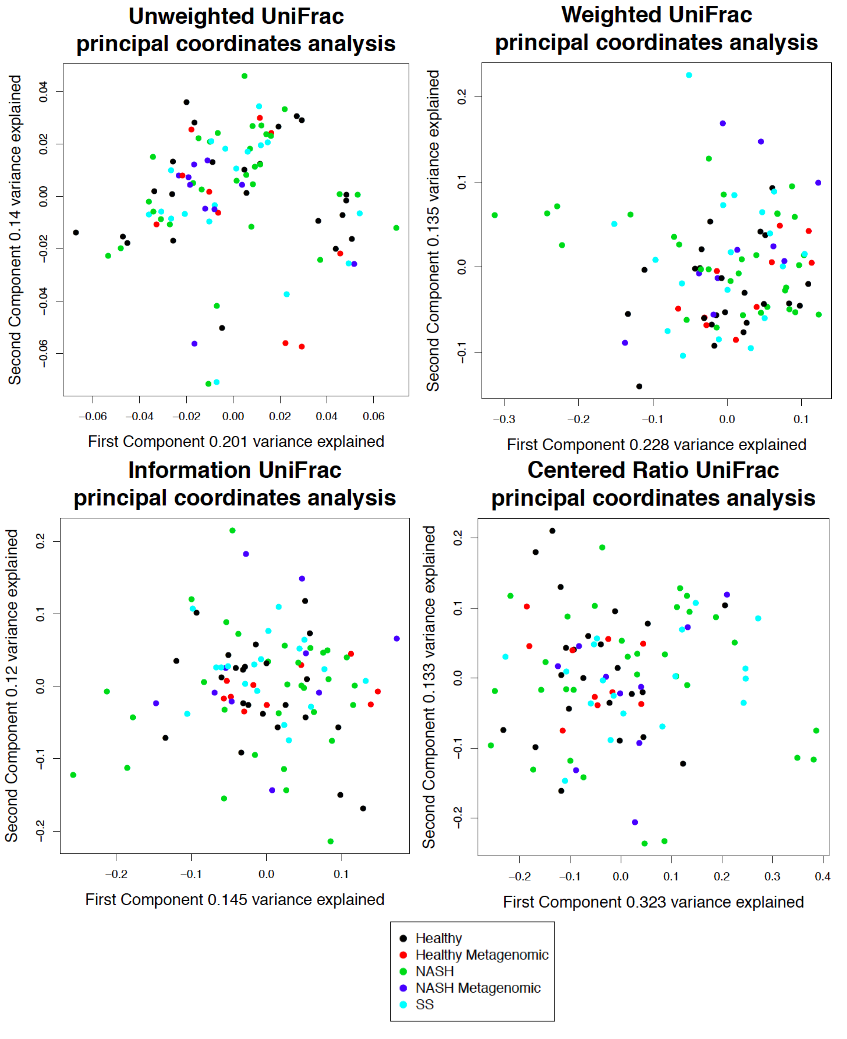
\includegraphics[width=0.95\textwidth]{nafld_16s_pcoa.png}
\caption[Principal Components Analysis of 16S rRNA gene tag sequencing data with different UniFrac weightings.]{\textbf{Principal Components Analysis of 16S rRNA gene tag sequencing data with different UniFrac weightings.} Each point represents one sample, and the distances between the samples have been calculated using different UniFrac metrics, taking into account phylogenetic as well as abundance information. There is no obvious separation between groups by any of the UniFrac weightings. Furthermore the variance explained by each principal component axis is not notably high, indicating a rather uniform data set.}
\end{center}
\label{nafld_fig2}
\end{figure}

\begin{figure}[h]
\begin{center}
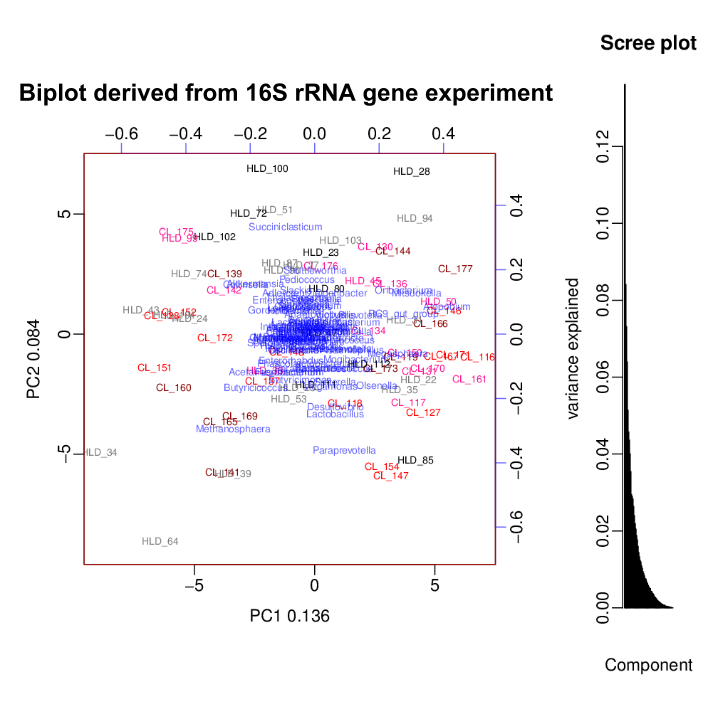
\includegraphics[width=0.95\textwidth]{nafld_16s_biplot.png}
\caption[16S rRNA gene tag sequencing experiment biplot.]{\textbf{16S rRNA gene tag sequencing experiment biplot.} Compositional data analysis is done by transforming the counts with a centered log ratio transform, and then performing a principal coordinate analysis. The variance explained by each genus is overlayed on the same principal coordinate analysis plot. Note that the variance explained by the first and the second coordinate is 9\% and 8\% respectively, indicating that there is not a clear unidirectional separation between groups. Samples from healthy controls are colored black while samples from patients with NASH are colored red. }
\end{center}
\label{nafld_16s_biplot}
\end{figure}

\begin{figure}[h]
\begin{center}
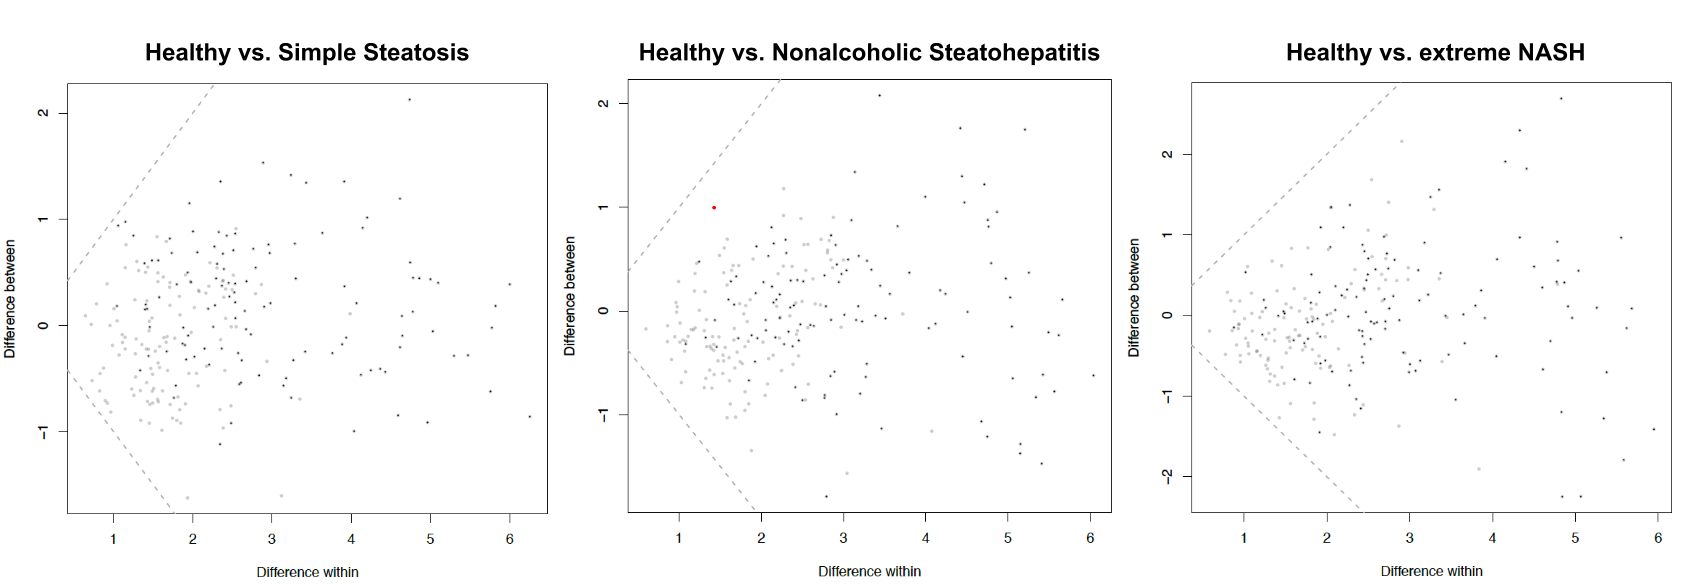
\includegraphics[width=0.95\textwidth]{nafld_16s_aldex.png}
\caption[Difference within vs. difference between groups.]{\textbf{Difference within vs. difference between groups.} Each point represents one OTU, and the differential abundance of that OTU within groups is plotted against the differential abundance between groups. None of the OTUs are more different between groups than within groups. The healthy samples used for these comparisons are the 10 healthy samples used for the metagenomic study. The extreme NASH samples used for these comparisons are the subset of the NASH patients selected for the metegenomic study.}
\end{center}
\label{nafld_fig3}
\end{figure}

When comparing all the healthy samples with all the NASH samples, the genus with the highest effect sizes are \textit{Adlercreutzia}, \textit{Odoribacter}, and \textit{Escherichia-Shigella}. However, when only the select 10 healthy samples and the 10 extreme NASH samples used in the metagenomic study are compared, the genus with the highest effect sizes are \textit{Ruminococcus}, \textit{Adlercreutzia}, and \textit{Alistipes}. This corresponds with the qPCR experiment, where \textit{Bacteriodetes}, \textit{Prevotella}, and \textit{Ruminococcus} were tested, and only \textit{Ruminococcus} was found to be differentially abundant.

\begin{figure}[h]
\begin{center}
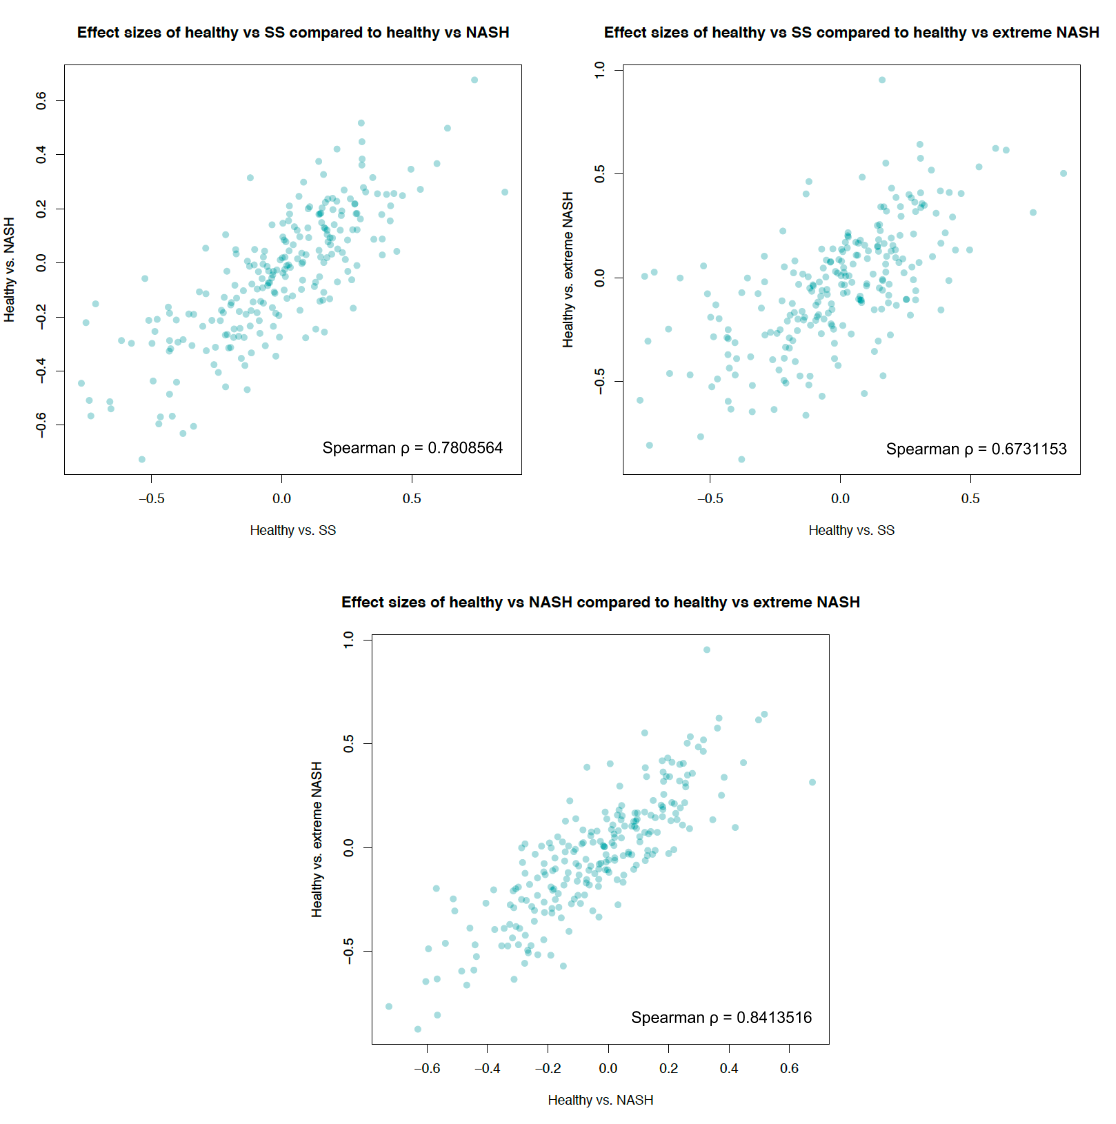
\includegraphics[width=0.95\textwidth]{nafld_16s_effect_sizes.png}
\caption[Correlation in effect sizes of different group experiments.]{\textbf{Correlation in effect sizes of different group experiments.} Each point represents one OTU, and the effect size of that OTU in one comparison (for example, comparing the gut microbiome of healthy patients with patients who have simple steatosis) is plotted against the effect size of that OTU in another comparison. The healthy samples used for these comparisons are the 10 healthy samples used for the metagenomic study. The extreme NASH samples used for these comparisons are the subset of the NASH patients selected for the metegenomic study. The median difference in the absolute effect sizes is -0.005547 for Healthy vs. NASH - Healthy vs. SS, 0.01094 for Healthy vs. extreme NASH - Healthy vs. SS, and 0.03105 for Healthy vs. extreme NASH - Healthy vs. NASH. The top decile of OTUs relatively increased in NASH for the metagenomic experiment are colored pink, and the top decile of OTUs relatively increased healthy for the metagenomic experiment are colored blue.}
\end{center}
\label{nafld_fig4}
\end{figure}

\FloatBarrier

A differential expression analysis performed with ALDEx2 between healthy vs. SS, healthy vs. NASH, and the 10 healthy samples selected for the metagenomic study vs. the 10 NASH samples for the metagenomic study yielded no significantly differentially abundant OTUs (Fig.~\ref{nafld_fig3}). However, the effect size (difference between groups divided by the difference within groups) of each OTU in each comparison is correlated (Fig.~\ref{nafld_fig4}). The effect sizes are higher in the Healthy vs. extreme NASH compared to the Healthy vs. SS or Healthy vs. NASH comparison.

\begin{table}[!ht]
% \begin{adjustwidth}{-2.25in}{0in} % Comment out/remove adjustwidth environment if table fits in text column.
\begin{tiny}
\begin{tabular}{|l|l|l|l|l|l|l|l|}
\hline
\bf{OTU family} & \bf{OTU genus} & \bf{SILVA} &\bf{H Vs. NASH} & \bf{H Vs. SS} & \bf{H vs. NASH} & \bf{16S genus} & \bf{MetaPhlAn}\\
& & \bf{bootstrap} & \bf{metagenomic} & \bf{effect sizes} & \bf{effect sizes} & \bf{effect sizes} & \bf{effect sizes}\\
& & \bf{value} & \bf{study effect sizes} & & & & \\ \hline
Acidaminococcaceae & Phascolarctobacterium & $100$ & $0.998$ & $0.122$ & $0.407$ & $0.827$ & $0.081$ \\ \hline
Lactobacillaceae & Lactobacillus & $97$ & $0.896$ & $0.534$ & $0.736$ & $0.587$ & $-0.899$ \\ \hline
Prevotellaceae & Paraprevotella & $100$ & $0.819$ & $0.208$ & $0.489$ & $0.843$ & $0.064$ \\ \hline
Lachnospiraceae & Incertae Sedis & $98$ & $0.673$ & $0.37$ & $0.2$ & NA & NA \\ \hline
Lachnospiraceae & Marvinbryantia & $77$ & $0.65$ & $0.159$ & $0.858$ & $0.077$ & $0.269$ \\ \hline
Lachnospiraceae & Incertae Sedis & $73$ & $0.634$ & $0.557$ & $0.32$ & NA & NA \\ \hline
Bifidobacteriaceae & Bifidobacterium & $100$ & $0.616$ & $0.262$ & $0.304$ & $0.188$ & $0.032$ \\ \hline
Ruminococcaceae & Incertae Sedis & $72$ & $0.586$ & $0.331$ & $0.291$ & NA & NA \\ \hline
Prevotellaceae & Paraprevotella & $100$ & $0.529$ & $0.691$ & $0.787$ & $0.843$ & $0.064$ \\ \hline
Lachnospiraceae & unclassified & $100$ & $0.505$ & $0.371$ & $0.571$ & NA & NA \\ \hline
unclassified & unclassified & $72$ & $0.505$ & $0.533$ & $0.244$ & NA & NA \\ \hline
Ruminococcaceae & Butyricicoccus & $71$ & $0.502$ & $0.198$ & $0.372$ & $0.449$ & $0.28$ \\ \hline
Lachnospiraceae & Incertae Sedis & $91$ & $0.5$ & $0.411$ & $0.339$ & NA & NA \\ \hline
Ruminococcaceae & Ruminococcus & $93$ & $0.494$ & $0.369$ & $0.253$ & $-0.866$ & $0.023$ \\ \hline
Coriobacteriaceae & unclassified & $97$ & $0.491$ & $0.334$ & $0.301$ & NA & NA \\ \hline
Lachnospiraceae & unclassified & $98$ & $0.478$ & $0.178$ & $0.341$ & NA & NA \\ \hline
Lactobacillaceae & Lactobacillus & $98$ & $0.476$ & $0.341$ & $0.439$ & $0.587$ & $-0.899$ \\ \hline
Ruminococcaceae & Subdoligranulum & $87$ & $0.475$ & $0.582$ & $0.483$ & $-0.087$ & $-0.177$ \\ \hline
Ruminococcaceae & Incertae Sedis & $98$ & $0.465$ & $0.939$ & $0.409$ & NA & NA \\ \hline
Ruminococcaceae & unclassified & $100$ & $0.462$ & $-0.4$ & $0.202$ & NA & NA \\ \hline
Coriobacteriaceae & Olsenella & $91$ & $0.443$ & $0.429$ & $0.183$ & $0.318$ & $0.141$ \\ \hline
Ruminococcaceae & Subdoligranulum & $98$ & $0.429$ & $0.245$ & $0.388$ & $-0.087$ & $-0.177$ \\ \hline
Lachnospiraceae & unclassified & $100$ & $0.429$ & $0.397$ & $0.342$ & NA & NA \\ \hline
Prevotellaceae & Prevotella & $99$ & $0.427$ & $0.111$ & $0.183$ & $0.212$ & $0.188$ \\ \hline
Lachnospiraceae & Anaerostipes & $100$ & $0.423$ & $0.298$ & $0.338$ & $0.244$ & $0.344$ \\ \hline
Prevotellaceae & unclassified & $70$ & $0.419$ & $0.203$ & $0.316$ & NA & NA \\ \hline
unclassified & unclassified & $92$ & $0.414$ & $0.136$ & $0.137$ & NA & NA \\ \hline
Ruminococcaceae & Incertae Sedis & $99$ & $0.412$ & $0.35$ & $0.473$ & NA & NA \\ \hline
Ruminococcaceae & Faecalibacterium & $100$ & $0.404$ & $0.185$ & $0.251$ & $-0.226$ & $-0.173$ \\ \hline
Alcaligenaceae & Sutterella & $100$ & $0.4$ & $0.177$ & $0.309$ & $0.162$ & $0.051$ \\ \hline
unclassified & unclassified & $73$ & $0.4$ & $0.345$ & $0.25$ & NA & NA \\ \hline
Rikenellaceae & Alistipes & $100$ & $0.397$ & $0.139$ & $0.17$ & $-0.687$ & $0.053$ \\ \hline
Lachnospiraceae & Roseburia & $98$ & $0.392$ & $0.612$ & $0.273$ & $0.18$ & $0.168$ \\ \hline
Prevotellaceae & unclassified & $75$ & $0.387$ & $0.131$ & $0.274$ & NA & NA \\ \hline
Coriobacteriaceae & Enterorhabdus & $72$ & $0.38$ & $0.029$ & $0.135$ & $0.429$ & $0.224$ \\ \hline
Ruminococcaceae & Ruminococcus & $100$ & $0.378$ & $0.146$ & $0.317$ & $-0.866$ & $0.023$ \\ \hline
unclassified & unclassified & $98$ & $0.366$ & $0.398$ & $0.275$ & NA & NA \\ \hline
Veillonellaceae & Dialister & $100$ & $0.353$ & $0.25$ & $0.145$ & $-0.297$ & $-0.038$ \\ \hline
Lachnospiraceae & unclassified & $100$ & $0.342$ & $-0.211$ & $0.301$ & NA & NA \\ \hline
Family XIII & Incertae Sedis & $100$ & $0.341$ & $0.295$ & $0.317$ & NA & NA \\ \hline
Bacteroidaceae & Bacteroides & $100$ & $0.333$ & $0.093$ & $0.201$ & $-0.356$ & $-0.124$ \\ \hline
Lachnospiraceae & unclassified & $100$ & $0.327$ & $0.155$ & $0.333$ & NA & NA \\ \hline
Lachnospiraceae & unclassified & $100$ & $0.327$ & $0.01$ & $0.214$ & NA & NA \\ \hline
Desulfovibrionaceae & Desulfovibrio & $100$ & $0.326$ & $-0.009$ & $-0.065$ & $0.283$ & $0.046$ \\ \hline
Lachnospiraceae & unclassified & $100$ & $0.309$ & $0.011$ & $0.117$ & NA & NA \\ \hline
Lachnospiraceae & Blautia & $96$ & $0.308$ & $0.218$ & $0.087$ & $-0.031$ & $0.192$ \\ \hline
Lachnospiraceae & Blautia & $97$ & $0.306$ & $-0.036$ & $0.215$ & $-0.031$ & $0.192$ \\ \hline
Ruminococcaceae & unclassified & $100$ & $0.305$ & $0.353$ & $0.462$ & NA & NA \\ \hline
Christensenellaceae & unclassified & $99$ & $0.303$ & $0.11$ & $0.277$ & NA & NA \\ \hline
Alcaligenaceae & Parasutterella & $100$ & $0.302$ & $0.252$ & $0.308$ & $0.389$ & $0.521$ \\ \hline
Lachnospiraceae & Incertae Sedis & $100$ & $0.3$ & $0.052$ & $0.153$ & NA & NA \\ \hline
Ruminococcaceae & Subdoligranulum & $92$ & $0.299$ & $0.056$ & $0.076$ & $-0.087$ & $-0.177$ \\ \hline
Acidaminococcaceae & Acidaminococcus & $100$  & $0.295$ & $0.287$ & $0.006$ & $0.345$ & $-0.737$ \\ \hline
\end{tabular}
\end{tiny}
\caption[Top decile of OTUs relatively increased in NASH based on effect size from healthy vs. NASH comparison.]{ \textbf{Top decile of OTUs relatively increased in NASH based on effect size from healthy vs. NASH comparison.} This table lists the OTUs, their effect sizes in all the comparisons, as well as the corresponding genus-level effect sizes in the 16S rRNA gene tag experiment and MetaPhlAn comparisons between the 10 healthy and 10 NASH samples selected for the metagenomic study. The OTUs were picked by open reference, by clustering and comparison with the SILVA database \cite{quast2013silva}. Positive effect sizes indicate that the feature was found to be relatively increased in NASH while negative effect sizes indicate that the featuer was found to be relatively increased in healthy. OTUs were annotated with SILVA, and a confidence percentage is reported based on the provided bootstrapping algorithm. \textit{Incertae Sedis} and unclassified genera were not analyzed at the genus level.}
\label{nafld_top_otu_table}
% \end{adjustwidth}
\end{table}

\begin{table}[!ht]
% \begin{adjustwidth}{-2.25in}{0in} % Comment out/remove adjustwidth environment if table fits in text column.
\begin{tiny}
\begin{tabular}{|l|l|l|l|l|l|l|l|}
\hline
\bf{OTU family} & \bf{OTU genus} & \bf{SILVA} &\bf{H Vs. NASH} & \bf{H Vs. SS} & \bf{H vs. NASH} & \bf{16S genus} & \bf{MetaPhlAn}\\
& & \bf{bootstrap} & \bf{metagenomic} & \bf{effect sizes} & \bf{effect sizes} & \bf{effect sizes} & \bf{effect sizes}\\
& & \bf{value} & \bf{study effect sizes} & & & & \\ \hline
Ruminococcaceae & Incertae Sedis & $100$ & $-0.349$ & $-0.539$ & $-0.411$ & NA & NA \\ \hline
Verrucomicrobiaceae & Akkermansia & $100$ & $-0.35$ & $-0.169$ & $-0.433$ & $-0.496$ $0.343$ & \\ \hline
Porphyromonadaceae & Parabacteroides & $100$ & $-0.35$ & $-0.529$ & $-0.349$ & $-0.313$ $0.016$ & \\ \hline
Rikenellaceae & Alistipes & $100$ & $-0.356$ & $-0.534$ & $-0.208$ & $-0.687$ $0.053$ & \\ \hline
Lachnospiraceae & Incertae Sedis & $73$ & $-0.36$ & $-0.392$ & $-0.173$ & NA & NA \\ \hline
Lachnospiraceae & unclassified & $100$ & $-0.361$ & $-0.549$ & $-0.411$ & NA & NA \\ \hline
Streptococcaceae & Streptococcus & $100$ & $-0.363$ & $-0.245$ & $-0.24$ & $-0.18$ $0.233$ & \\ \hline
Lachnospiraceae & unclassified & $100$ & $-0.369$ & $-0.082$ & $-0.169$ & NA & NA \\ \hline
Lachnospiraceae & Dorea & $100$ & $-0.369$ & $-0.241$ & $-0.252$ & $-0.267$ $-0.154$ & \\ \hline
Lachnospiraceae & Roseburia & $83$ & $-0.371$ & $0.019$ & $-0.507$ & $0.18$ $0.168$ & \\ \hline
Lachnospiraceae & Incertae Sedis & $82$ & $-0.379$ & $-0.3$ & $-0.424$ & NA & NA \\ \hline
Christensenellaceae & unclassified & $98$ & $-0.386$ & $-0.051$ & $-0.14$ & NA & NA \\ \hline
Christensenellaceae & unclassified & $100$ & $-0.387$ & $-0.571$ & $-0.467$ & NA & NA \\ \hline
Lachnospiraceae & Blautia & $93$ & $-0.387$ & $-0.704$ & $-0.532$ & $-0.031$ $0.192$ & \\ \hline
Ruminococcaceae & unclassified & $100$ & $-0.393$ & $-0.511$ & $-0.2$ & NA & NA \\ \hline
Lachnospiraceae & Roseburia & $91$ & $-0.397$ & $-0.568$ & $-0.603$ & $0.18$ $0.168$ & \\ \hline
Porphyromonadaceae & Odoribacter & $100$ & $-0.397$ & $0.005$ & $-0.135$ & $-0.541$ $-0.333$ & \\ \hline
Lachnospiraceae & Incertae Sedis & $85$ & $-0.397$ & $-0.265$ & $-0.362$ & NA & NA \\ \hline
Lachnospiraceae & unclassified & $98$ & $-0.401$ & $-0.135$ & $-0.289$ & NA & NA \\ \hline
Porphyromonadaceae & Odoribacter & $100$ & $-0.422$ & $-0.625$ & $-0.492$ & $-0.541$ $-0.333$ & \\ \hline
Erysipelotrichaceae & Turicibacter & $100$ & $-0.424$ & $-0.206$ & $-0.251$ & $-0.52$ $-0.717$ & \\ \hline
Christensenellaceae & unclassified & $100$ & $-0.443$ & $-0.452$ & $-0.329$ & NA & NA \\ \hline
Ruminococcaceae & Ruminococcus & $100$ & $-0.444$ & $-0.429$ & $-0.282$ & $-0.866$ $0.023$ & \\ \hline
Christensenellaceae & unclassified & $99$ & $-0.445$ & $-0.602$ & $-0.464$ & NA & NA \\ \hline
Lachnospiraceae & unclassified & $100$ & $-0.452$ & $-0.387$ & $-0.564$ & NA & NA \\ \hline
Bacteroidaceae & Bacteroides & $100$ & $-0.456$ & $-0.038$ & $-0.4$ & $-0.356$ $-0.124$ & \\ \hline
Ruminococcaceae & Incertae Sedis & $84$ & $-0.461$ & $-1.024$ & $-0.668$ & NA & NA \\ \hline
Veillonellaceae & Dialister & $100$ & $-0.479$ & $0.036$ & $-0.405$ & $-0.297$ $-0.038$ & \\ \hline
Bacteroidaceae & Bacteroides & $100$ & $-0.488$ & $-0.534$ & $-0.521$ & $-0.356$ $-0.124$ & \\ \hline
Prevotellaceae & Alloprevotella & $100$ & $-0.5$ & $-0.667$ & $-0.172$ & $-0.001$ $0.863$ & \\ \hline
Bacteroidaceae & Bacteroides & $100$ & $-0.502$ & $-0.487$ & $-0.272$ & $-0.356$ $-0.124$ & \\ \hline
Rikenellaceae & Alistipes & $100$ & $-0.517$ & $-0.369$ & $-0.367$ & $-0.687$ $0.053$ & \\ \hline
Coriobacteriaceae & Adlercreutzia & $100$ & $-0.521$ & $-0.309$ & $-0.452$ & $-0.372$ $-0.298$ & \\ \hline
Ruminococcaceae & unclassified & $100$ & $-0.522$ & $-0.571$ & $-0.436$ & NA & NA \\ \hline
Family XIII & Anaerovorax & $91$ & $-0.533$ & $-0.611$ & $-0.624$ & $-0.476$ $-0.152$ & \\ \hline
Ruminococcaceae & unclassified & $76$ & $-0.54$ & $-0.59$ & $-0.573$ & NA & NA \\ \hline
Lachnospiraceae & Pseudobutyrivibrio & $98$ & $-0.543$ & $-0.712$ & $-0.46$ & $-0.423$ $-0.091$ & \\ \hline
Bacteroidaceae & Bacteroides & $100$ & $-0.546$ & $-0.766$ & $-0.647$ & $-0.356$ $-0.124$ & \\ \hline
Bacteroidaceae & Bacteroides & $100$ & $-0.561$ & $-0.069$ & $-0.184$ & $-0.356$ $-0.124$ & \\ \hline
Lachnospiraceae & Blautia & $85$ & $-0.562$ & $-0.906$ & $-0.561$ & $-0.031$ $0.192$ & \\ \hline
Ruminococcaceae & Faecalibacterium & $100$ & $-0.566$ & $-0.704$ & $-0.724$ & $-0.226$ $-0.173$ & \\ \hline
unclassified & unclassified & $85$ & $-0.601$ & $-0.381$ & $-0.382$ & NA & NA \\ \hline
Ruminococcaceae & Incertae Sedis & $100$ & $-0.63$ & $-0.463$ & $-0.635$ & NA & NA \\ \hline
Ruminococcaceae & Subdoligranulum & $99$ & $-0.636$ & $-0.523$ & $-0.422$ & $-0.087$ $-0.177$ & \\ \hline
Ruminococcaceae & Incertae Sedis & $97$ & $-0.668$ & $-0.544$ & $-0.565$ & NA & NA \\ \hline
Ruminococcaceae & Ruminococcus & $100$ & $-0.669$ & $-0.516$ & $-0.591$ & $-0.866$ $0.023$ & \\ \hline
Lachnospiraceae & Incertae Sedis & $85$ & $-0.67$ & $-0.532$ & $-0.686$ & NA & NA \\ \hline
Lachnospiraceae & Coprococcus & $91$ & $-0.686$ & $-0.733$ & $-0.577$ & $-0.647$ $0.469$ & \\ \hline
Ruminococcaceae & unclassified & $74$ & $-0.725$ & $-0.533$ & $-0.658$ & NA & NA \\ \hline
Erysipelotrichaceae & unclassified & $100$ & $-0.736$ & $-0.621$ & $-0.83$ & NA & NA \\ \hline
Ruminococcaceae & Subdoligranulum & $85$ & $-0.746$ & $-0.594$ & $-0.581$ & $-0.087$ $-0.177$ & \\ \hline
Lachnospiraceae & Dorea & $100$ & $-0.759$ & $-0.94$ & $-0.554$ & $-0.267$ $-0.154$ & \\ \hline
Family XIII & Incertae Sedis & $91$ & $-0.985$ & $-0.563$ & $-0.622$ & NA & NA \\ \hline
\end{tabular}
\end{tiny}
\caption[Bottom decile of OTUs relatively increased in healthy based on effect size from healthy vs. NASH comparison.]{ \textbf{Bottom decile of OTUs relatively increased in healthy based on effect size from healthy vs. NASH comparison.} This table lists the OTUs, their effect sizes in all the comparisons, as well as the corresponding genus-level effect sizes in the 16S rRNA gene tag experiment and MetaPhlAn comparisons between the 10 healthy and 10 NASH samples selected for the metagenomic study. The OTUs were picked by open reference, by clustering and comparison with the SILVA database \cite{quast2013silva}. Positive effect sizes indicate that the feature was found to be relatively increased in NASH while negative effect sizes indicate that the featuer was found to be relatively increased in healthy. OTUs were annotated with SILVA, and a confidence percentage is reported based on the provided bootstrapping algorithm. \textit{Incertae Sedis} and unclassified genera were not analyzed at the genus level.}
\label{nafld_bot_otu_table}
% \end{adjustwidth}
\end{table}


\FloatBarrier

\subsection{Metagenomic experiment}

\paragraph{MetaPhlAn}\mbox{}\\

We ran the metagenomic sequences through MetaPhlAn to infer what the results would be with 16S rRNA gene tag sequencing, so that we could compare with our empirical 16S rRNA gene tag sequencing results. The effect size Spearman coefficient (Fig.~\ref{nafld_metaphlan_effect}) is smaller than the effect size coefficient between the healthy vs. SS and healthy vs. NASH comparison, even though in this case the same samples are being compared.

The operational taxonomic units in the MetaPhlAn and 16S rRNA gene analysis were derived from different databases, and could not be compared directly, so the effect size comparison in Fig.~\ref{nafld_metaphlan_effect} was done at the genus level. Note that OTUs can reside in between genuses, such that the genus classificaiton is not perfectly concordant between the two comparisons. The top four relatively abundant genera from the MetaPhlAn analysis were \textit{Ruminococcus}, \textit{Eubacterium}, \textit{Coprococcus}, and \textit{Bacteroides}. Only \textit{Bacteroides} is also on the top four relatively abundant genera from the 16S rRNA gene tag sequencing experiment.

\begin{figure}[h]
\begin{center}
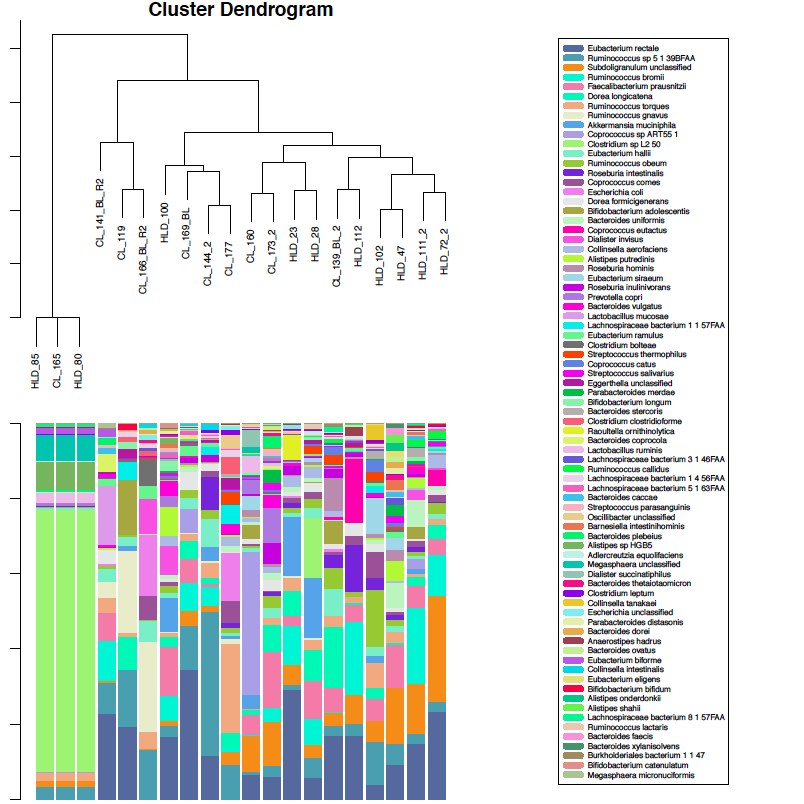
\includegraphics[width=0.95\textwidth]{metaphlan_barplot_dendogram.png}
\caption[Taxa barplot dendogram derived from MetaPhlAn.]{\textbf{Taxa barplot dendogram derived from MetaPhlAn.} The metagenomic reads were input into MetaPhlAn to generate a count table. The taxa in the count table were filtered such that only taxa with at least 1\% abundance in any sample was kept. In this barplot, each bar represents one sample, and each color represents one genus, with the size of the colored segments corresponding with the relative abundance of the genus.}
\end{center}
\label{nafld_metaphlan_barplot}
\end{figure}

\begin{figure}[h]
\begin{center}
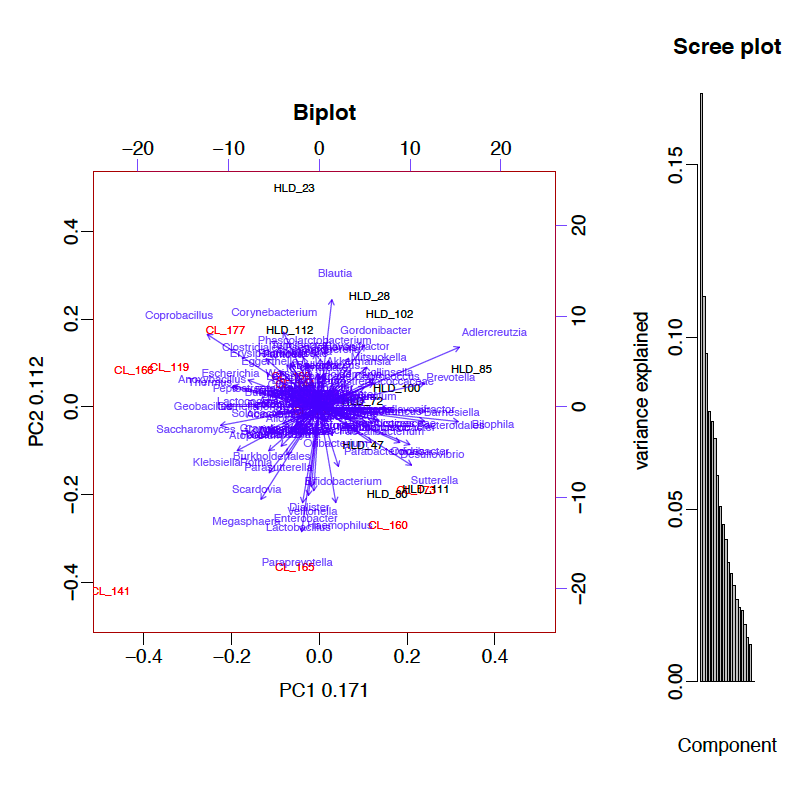
\includegraphics[width=0.95\textwidth]{metaphlan_biplot.png}
\caption[Biplot derived from MetaPhlAn.]{\textbf{Biplot derived from MetaPhlAn.} Compositional data analysis is done by transforming the counts with a centered log ratio transform, and then performing a principal coordinate analysis. The variance explained by each genera is overlayed on the same principal coordinate analysis plot. This biplot was generated from the count table inferred by MetaPhlAn, with taxa filtered such that only taxa with at least 1\% abundance in any sample was kept. Note that the variance explained by the first and the second coordinate is 17\% and 11\% respectively, indicating that there is not a clear unidirectional separation between groups. Samples from healthy controls are colored black while samples from patients with NASH are colored red.}
\end{center}
\label{nafld_metaphlan_biplot}
\end{figure}

\begin{figure}[h]
\begin{center}
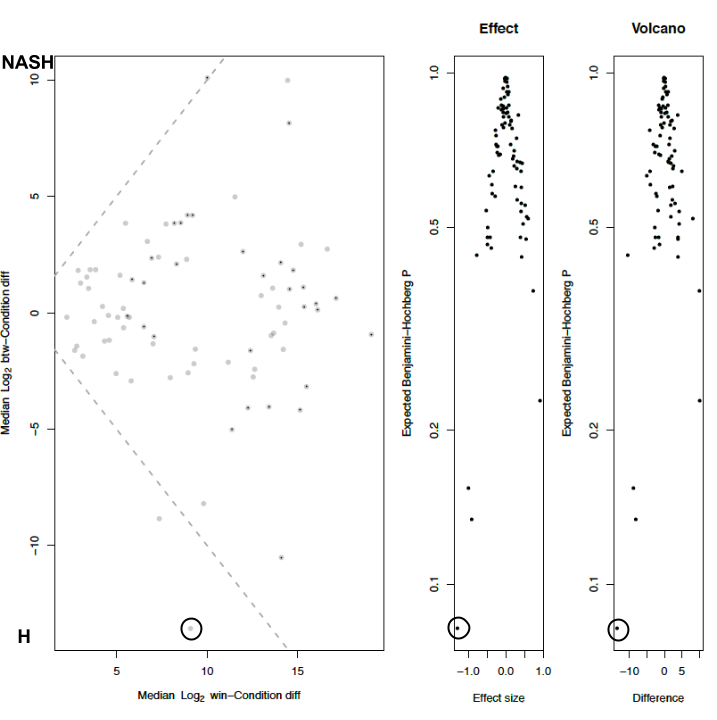
\includegraphics[width=0.95\textwidth]{metaphlan_aldex.png}
\caption[Difference within groups vs. difference between groups per taxa, derived from MetaPhlAn.]{\textbf{Difference within groups vs. difference between groups per taxa, derived from MetaPhlAn.} This plot was generated from the count table inferred by MetaPhlAn, with taxa filtered such that only taxa with at least 1\% abundance in any sample was kept. No taxa are more differential between groups than within groups. A positive difference between indicates that the taxa was relatively increased in NASH while a negative difference between indicates that the taxa was relatively increased in healthy. This analysis was done at the OTU level.}
\end{center}
\label{nafld_metaphlan_aldex}
\end{figure}

\begin{figure}[h]
\begin{center}
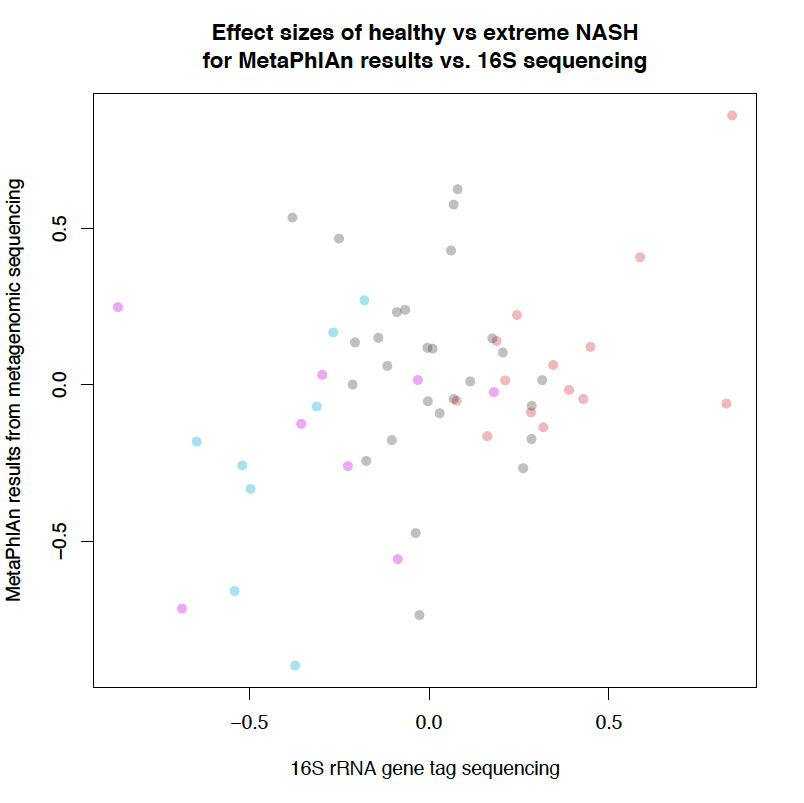
\includegraphics[width=0.95\textwidth]{metaphlan_16s_effects.png}
\caption[Effect size correlation between MetaPhlAn and 16S rRNA gene tag sequencing.]{\textbf{Effect size correlation between MetaPhlAn and 16S rRNA gene tag sequencing.} For this plot, taxa were amalgamated at the genus level. The effect sizes for the comparison of the healthy and NASH samples selected for the metagenomic study are shown. The Spearman coefficient is 0.2021001. Genera corresponding with OTUs identified to have the top deciles of effect sizes in the 16S rRNA gene tag experiment comparison are colored - red for OTUs relatively abundant in NASH, and blue for OTUs relatively abundant in the healthy condition. Genera corresponding to both OTUs in the NASH and healthy deciles are colored purple.}
\end{center}
\label{nafld_metaphlan_effect}
\end{figure}

\FloatBarrier

\section{Discussion}

Given the inconsistency in the five papers that have been published about NAFLD and the gut microbiome, we have performed our analysis in a rigorous manner in an effort to find OTUs with true effects. We found that there was no significant difference between groups by sample clustering (Fig.~\ref{nafld_fig2}) or at the level of the individual OTUs (Fig.~\ref{nafld_fig3}).

There are several factors that would make such a study underpowered. First, the gut microbiome is highly diverse between individuals. This is compounded by the fact that the samples were taken from a diverse Toronto population, including people who immigrated from other countries who likely have different diets. The literature shows that differences in the gut microbiome are often driven by diet \cite{david2014diet}. Additionally, the nature of microbiome data is that there are very many more variables (in the form of OTUs or annotated gene functions) than samples, and the power of the study is inversely proportional to the number of variables.

From Fig.~\ref{nafld_fig4}, the correlation shows that even though there is not enough power to detect a significant difference, the difference from the healthy baseline are moving in the same direction through simple steatosis to nonalcoholic steatohepatitis to extreme NASH.

We hypothesize that there is a characterizable difference in the gut microbiome between patients prone to NASH and healthy controls. Further study with a higher sample size, a more homogenous population, and a greater phenotypic difference between groups may provide the statistical power required to detect the nature of this difference.
